\documentclass[letterpaper,10pt]{article}
\usepackage[utf8x]{inputenc}
\usepackage{graphicx,color}

% Construct the basic page sizes
\oddsidemargin  0.0in
\evensidemargin 0.0in
\textwidth      6.5in
\headheight     0.5in
\topmargin      0.0in
\textheight=8.5in

\usepackage{fancyhdr}

\pagestyle{fancyplain} { % define first page header and footer
\fancyhead[C]{\textit{\Large{DRAFT Specification}}\\}
}

%opening
\title{Event Location Components for GMAT}
\author{Darrel J. Conway\\\emph\small{{Thinking Systems, Inc.}}}

\begin{document}

\maketitle

\begin{abstract}
This document describes the components used in the event location subsystem of
the General Mission Analysis Tool (GMAT).  The document is written in a style
that facilitates inclusion in GMAT's Architectural Specification.
\end{abstract}

\section{Overview}

The event location subsystem in GMAT is used to detect the start and end times
for various events of interest to the mission analysts designing or flying a
mission.  This subsystem locates the event boundaries, consolidates them into
reports accessible to the users, and provides event data for use inside of
GMAT's Mission Control Sequence.

GMAT's event location subsystem is based on the event location algorithms
described in reference~\cite{pip}.  The subsystem consists of event locator
classes, event function calculators, root detector algorithms and finders, and
interfaces to other GMAT subsystems, most notably the propagation subsystem.  

The event functions are defined analytically to have roots (function zeroes) at
the event boundaries and analytic, continuous first derivatives.  The event
function derivatives are passed to the propagation system for use in step
size control to ensure that propagation steps avoid stepping over multiple
event boundaries in a single step.  The root detector is built into the
propagation system, and used to determine when one or more potential root
boundaries have occurred during a propagation step.  

If an event boundary is detected in the propagation interval, the propagation
data is buffered and control is passed to a method that located the boundary,
using a root finding algorithm to search for and locate each root in the
propagation step. This root location is performed by propagating to the epoch of
the root candidate and evaluating the event function, iterating on the process
until either a root is located to a specified tolerance or the algorithm
determines that the potential root does not actually exist in the propagation
interval.

This overview of the root location process is, of necessity, sketchy and omits
many of the details of the implemented process.  Interested readers are
referred to reference~\cite{aasastro} for details of the algorithm.  The
following sections describe the design of the system in GMAT.

\section{Class Overview}

\begin{figure}
\begin{center}
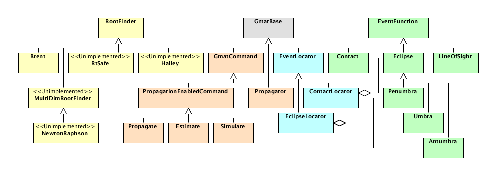
\includegraphics[scale=2.0]{./Images/EventLocationClasses.eps}
\caption{\label{fig:EventClasses}Classes Implementing GMAT's Event Location
Subsystem}
\end{center}
\end{figure} 

Figure~\ref{fig:EventClasses} shows the classes used in the event location
subsystem.  The classes in the figure fall into four categories: the 
propagation classes that control the detection and location process, RootFinder
classes, EventLocator classes, and EventFunction classes.  Two of these
categories, PropagationEnabledCommands and RootFinders, are classes that operate
closely with the propagation subsystem when a Mission Control Sequence is run in
GMAT.  The EventLocator classes provide the user interface into the event
location subsystem, and supports the scripting that activates the subsystem. 
The EventFunction classes provide the detailed computations needed to evaluate
the status of a specific spacecraft state relative to an event under
consideration.  The location classes are described in more detail later in this
document, along with the elements of the commands that drive the event location
process. 

\section{The Event Location Process} 

The following sections describe the scripting, initialization, and execution of
the event location subsystem in GMAT.

\subsection{Scripting Event Location}

Event location is activated in GMAT by creating an EventLocator object of the
type desired for the mission being designed.  From either GMAT's Graphical User
Interface (GUI) or in a script file, the user creates a new EventLocator object
and sets its parameters according to the mission's requirements.  Details of the
GUI configuration are outside of the scope of this document.  An example of the
serialized version of this configuration, captured in the scripting for event
location, is presented here:

\begin{quote}
\begin{verbatim}
Create Spacecraft sat;
...
Create EclipseLocator ecl;
ecl.Spacecraft = {sat};
ecl.OccultingBodies = {Earth, Luna};
ecl.Tolerance = 1e-7;
ecl.Filename = SatEclipseData.report;
ecl.ShowPlot = true;
...
Create Propagator prop;
...
BeginMissionSequence
Propagate prop(sat) {sat.ElapsedDays = 7};
Toggle ecl Off;
Propagate prop(sat) {sat.ElapsedDays = 7};
Toggle ecl On;
Propagate prop(sat) {sat.ElapsedDays = 7};
\end{verbatim}
\end{quote}

\noindent When this script is run, GMAT propagates the spacecraft named sat for
21 days.  It collects event data for Earth and Moon (Luna) shadow entry and exit
for the umbra, penumbra, and antumbra shadow regions during the first and last
seven days of propagation, but does not collect event data during the middle
seven days of propagation.  These data are written to a report file named
``SatEclipseData.report'' and shown in a scatter plot at the end of the run. 
The following paragraphs describe the internal workings of GMAT to accomplish
this task. 

\subsection{Initializing the Event Location Components}

The event location subsystem follows the normal initialization process in GMAT.
 Objects created in the script or GUI are stored in GMAT's Configuration for
use during a run.  When a script is run, the objects are cloned from the
configuration into the Sandbox used for the run.  These objects are asked for
their lists of referenced objects, and the corresponding pointers returned to
the objects.  Finally, each object's Initialize() method is called so that
interconnections and other settings needed to run the mission can be
established.

For the event location subsystem, the bulk of the initialization occurs in the
Mission Control Sequence initialization after the Sandbox has received and
initialized the clones of the configuration objects.  The control sequence
initialization sets the connections between event locators and the commands
that use them.  

Both of these initialization steps are described below.

\subsubsection{Initialization for the Event Locator}

Pointers to referenced objects in the Sandbox For the EventLocators are set
before the locators are initialized. Each EventLocator manages one or more
EventFunctions designed to evaluate to zero at event boundaries, to a positive
number while the event is occurring, and to a negative number outside of the
event.  The initialization process for the EventLocators consists of passing
reference object pointers to the EventFunctions and then calling the
Initialize() method on each event function.  Each EventFunction tests the object
pointers to be sure that they are compatible with the function calculations and
to ensure that all needed objects have been set, and then reports that it is
ready for use to the EventLocator that manages it.

Once the EventLocator objects are initialized, the Sandbox collects the
EventLocators into an std::vector container.  This vector is passed to each
command in the Mission Control Sequence during command initialization.

\subsubsection{Initialization in the Mission Control Sequence}

The initialization for the EventLocator classes, described above, is
straightforward and all performed when a mission is loaded into one of GMAT's
Sandboxes.  That initialization is a first step in the complete initialization
process.  The Sandbox uses the configured EventLocator object clones in its
Sandbox Object Map to build a vector of EventLocator objects for use by the
commands.  This vector is passed to the commands when the mission control
sequence is initialized.  Commands that work with events use the vector as the
source of the event data objects.  

\begin{figure}
\begin{center}
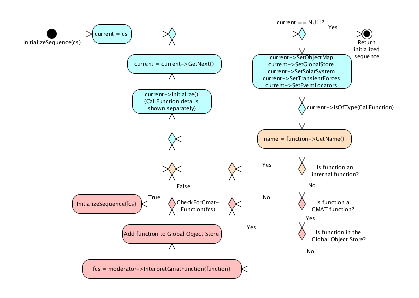
\includegraphics[scale=1.7]{./Images/InitializeMCS.eps}
\caption{\label{fig:InitializeMCS}Mission Control Sequence Initialization}
\end{center}
\end{figure} 

Figure~\ref{fig:InitializeMCS} shows the initialization process for the Mission
Control Sequence in the Sandbox.  The EventLocator vector is passed to each
command in the Mission Control Sequence, as is indicated in the first activity
bubble in the initialization loop.  Commands that do not use this vector simply
discard the vector pointer.  During the run, each command that uses the event
vector retrieves pointers to the needed EventLocators from the vector and uses
them to access the event locator and event function components.  An example of
this usage in the Propagate command is described next.

\subsection{Event Location During a Run}

Each EventLocator has a Boolean flag indicating if its event calculations are
active in the Mission Control Sequence.  The RootDetector uses this flag to
track the event calculations that need to be performed during execution of the
control sequence. As was described in the initialization section, each command
in the control sequence has a copy of the vector of event locators defined in
the Sandbox.  Commands that use the event data access the data through the
pointers contained in this vector.  

The propagation enabled commands are prime candidates for this usage because
they use the event locator structures to determine when an event candidate
occurs and to search for the event start and end times.  As an example, 
Figure~\ref{fig:PropagateWithEvents} shows the control flow in the Propagate
command when events are present in the Mission Control Sequence.  The flow
through execution of the propagate command in the absence of event location
elements can be seen in GMAT's Architectural Specification~\cite{archspec}. The
activity diagram in Figure~\ref{fig:PropagateWithEvents} updates the control
flow in the Propagate command with event location calls, shown in orange on the
figure.   

\begin{figure}
\begin{center}
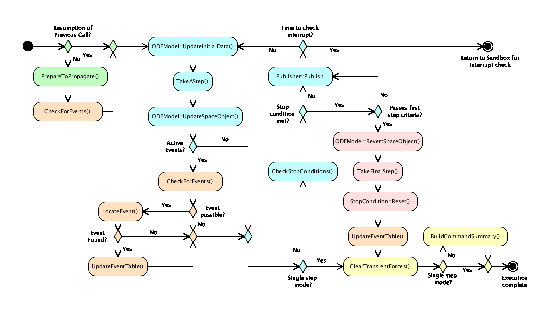
\includegraphics[scale=1.7]{./Images/ExecutePropEvents.eps}
\caption{\label{fig:PropagateWithEvents}Control Flow for the Propagate
Command with Events}
\end{center}
\end{figure} 

Each propagation enabled command begins execution by calling the
PrepareToPropagate() method, which constructs the class linkages necessary for
propagation, builds the state vector that is propagated, and fills that
propagation state vector with the data used at the start of propagation.  The
initial event function values are set in a call to the Initialize() method made
from this call.  That call prepares the Propagators for all time evolution of
the data contained in the state vector. It also initializes the data structures
needed for event location, so that event detection can proceed.  GMAT's event location algorithm requires that the event functions be integrated along with the other forces in the force model during propagation. The addition of event location to a mission also adds the derivative of the event functions to the propagation state vector, so that the event function evolution can be used as part of the criteria involved in determining the propagation step size for a step taken by a numerical integrator.  This new addition to the ODE model is made through the EventModel class, described below.

Analytic integrators employ a similar mechanism.  They load the initial event
data into the location buffers during a call to initialization method, and set
up data structures designed to ensure that they avoid steps too large for
effective event location. The details for the implementation of step size
control in the analytic propagators are TBD.

Before taking a propagation step, the propagation enabled command ensures that
its root detection data structures contain the initial event values by calling
the InitializeForEventLocation() method.  That method, called in the
initialization process described above, evaluates each active event in the vector
of EventLocators and stores the resulting event function values in a buffer in
the PropagationEnabledCommand.  Once this task is accomplished, the command
continues with propagation as designed, updating potentially changing ancillary
data for the force model (items like the current total mass of the spacecraft,
area data, and so forth) and then taking a propagation step and passing the
updated data to the objects that are being propagated.  At that point, all of
the data generated by propagation is passed back to the objects being
propagated.

Once the propagated objects are updated, The command checks to see if there are
any active events. If active events exist, the propagated data is checked
for events occurring in the propagation interval.  If there are potential
events in that span, they are located and the event data is stored in the
EventLocator.  Details of this process will be specified shortly.  After
any needed event location has been performed, the propagation stopping
conditions are evaluated, data is sent to the Subscribers that need it, and
propagation continues if no stops were triggered, or is finalized if a stopping
condition was encountered.

If a stopping condition was encountered, the propagation advances to the
stopping condition, and then passes the resulting data to the event subsystem so
that detected events that occur in the raw propagation step but outside of the
step to the stopping condition can be removed from the EventLocator's event
table.

\begin{figure}[htb]
\begin{center}
\includegraphics[scale=1.6]{./Images/ProcessEvents.eps}
\caption{\label{fig:ProcessEvents}The Event Location Process}
\end{center}
\end{figure} 

Figure~\ref{fig:ProcessEvents} shows the details of event location in a
propagation enabled command, using the Propagate command as an example.  Once
the command has taken a propagation step and updated the propagated objects, it
calls the CheckForEvents(), defined in the PropagationEnabledCommand base
class.  (The CheckForEvents() method and associated calls is shown in the figure
using the green lifeline.) That code evaluates each active EventLocator, which
in turn evaluates each of its EventFunctions. The event function values and
derivative values are then checked to see if there is a potential event in the
propagation interval. Events are found either through a sign change in the value
of the corresponding event function, bracketing the event in the propagation
interval, or through a change in sign of the event function derivative,
indicating that there is the potential for two events in the propagation
interval.  The alternative of many potential events in the interval is precluded
by the form of the event function producing propagation step sizes compatible
with the potential event frequency, coupled with wise selection of propagation
parameters made by the user to preclude stepping across many events in a single
propagation step.

If an event is bracketed or a potential pair of events is detected, the
propagation system buffers the propagation states and other propagation
parameters and then begins the event location process. Control is passed to the
LocateEvent() method, shown in the figure using orange lifelines.  This method
examines the event function data and derivatives.  For each event function that
shows a sign change in either function or, with proper function values,
derivative data, the zero of that function or derivative is located. Function
zeroes identify event boundaries, and are passed to the event table for
reporting.  

When function derivative zeroes are found, the event function value at that
location is evaluated and compared to the function value at the epochs
bracketing the derivative zero.  If these comparisons show a sign change between
the bracketing points and the derivative zero location, the event function
zeroes in the bracketed intervals are located and added to the event table.

The LocateEvent() function begins by passing the bracketing data to a
RootFinder object, initializing that object.  The PropagationEnabledCommand then
enters a loop used to search for the zero bracketed by the initialization data.
The command requests a step from the root finder algorithm, propagates the
spacecraft by the requested amount, and updates the spacecraft data at that
epoch.  Then the event functions are evaluated, and the resulting values passed
back to the root finder.  The function data is then checked to see if the
search loop can terminate.  The loop ends when one of the following conditions
is met:

\begin{itemize}
\item The magnitude of the function or derivative value is less than the
tolerance set on the corresponding event locator.
\item  The number of search steps taken is more than the maximum number allowed
(currently set to 31).
\item The size of the requested step is smaller than the machine precision for
epoch data.
\end{itemize}
  
\noindent It is possible that the root finding algorithm does not find any
zeroes of the event function.  Data is only passed into the event table when a
zero is found; searches with null results do not add data to the event table. 

By default, GMAT uses Brent's method to determine the step to the next
evaluation point in the RootFinder code. The system design allows the inclusion
of other methods as needed, but the current implementation only provides Brent's
method.

\subsection{The EventModel Class}

Event location in GMAT is performed based on analytic event functions defined such that the function is continuous, differentiable, and evaluates to zero at event entry and exit points.  GMAT regulates its propagation adaptively to control integration steps so that the propagation steps do not skip over event pairs.  The event functions are inserted into the propagation through a class, the EventModel class, that collects event function data for the ODEModel.  EventModel instances are created in each PropagationEnabledCommand when that command is prepared for propagation, immediately before the ODEModel is used.  The process followed to set up the EventModel is shown in Figure~\ref{fig:InitializeForEventLocation}.  At the end of this process, the ODEModel for each PropSetup in the PropagationEnabledCommand owns an EventModel, configured to integrate the EventFunctions in each EventLocator that is active for the spacecraft associated with that PropSetup.  These EventModels are initialized with the rest of the ODEModel when the command executes its PrepareToPropagate method.

\begin{figure}[htb]
\begin{center}
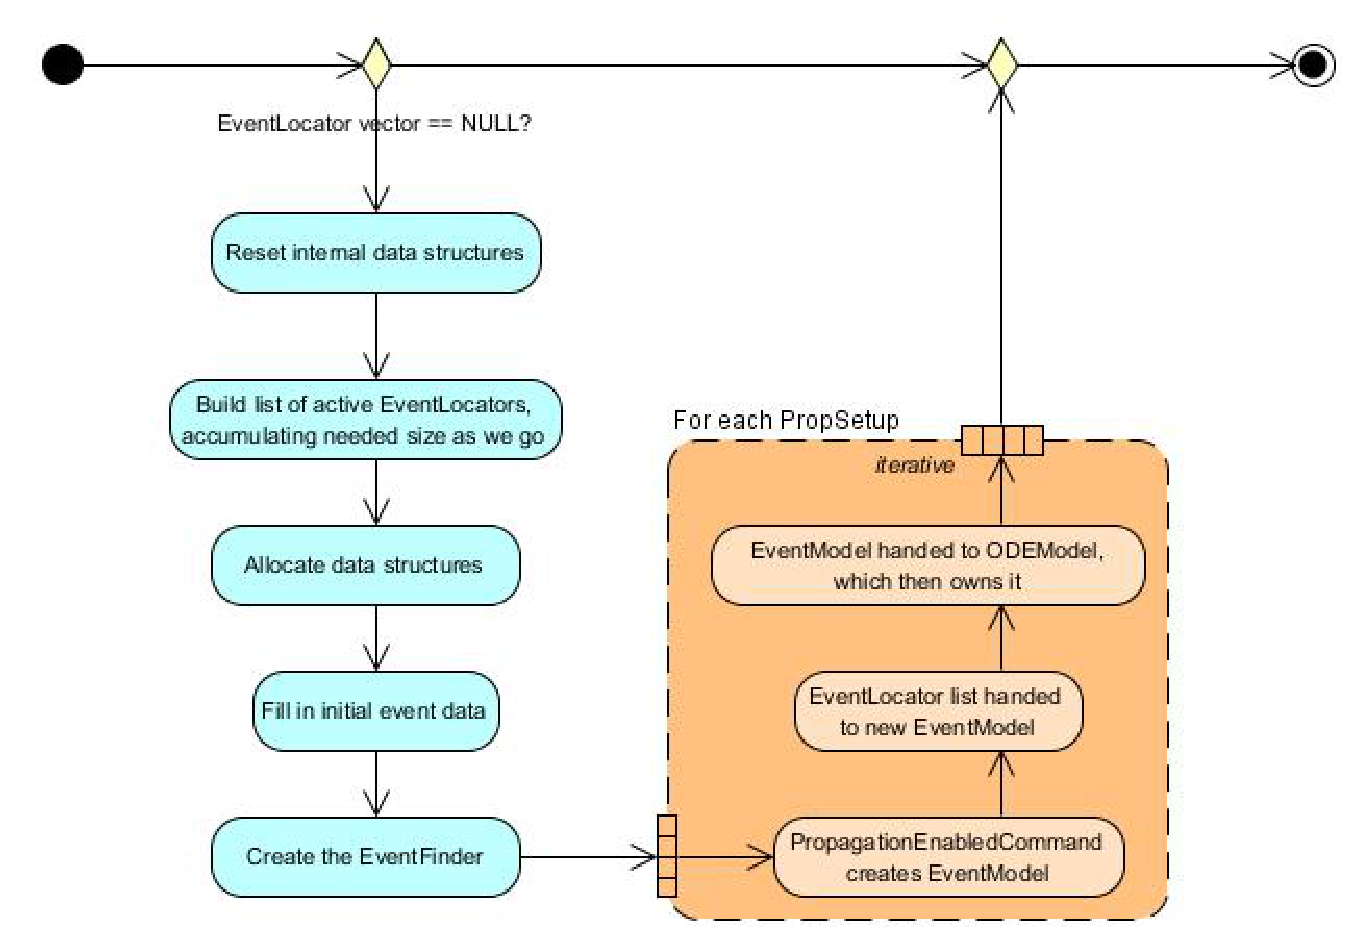
\includegraphics[scale=0.5]{./Images/InitializeForEventLocation.eps}
\caption{\label{fig:InitializeForEventLocation}Setting Up the EventModel}
\end{center}
\end{figure} 

During initialization, each EventModel object gathers data from the vector of event locators and sets up indices into the propagation state vector for each event function in the locators.  After collecting this data from each event locator, the index of associated data in the propagation state vector is passed to the locator for each event function so that the event function value can be computed during propagation.

During propagation, the event function data is loaded into the propagation state vector.  This data loading is accomplished by looping through the event locators, evaluating each in turn.  The resulting derivative data is placed into the model's local derivative vector.  That vector, in turn, is used by the ODEModel when building the superposition data that is returned to the integrator.

\section{Locator Class Details}

The initialization and execution descriptions above dictate some key structures
in the classes that compose the event location subsystem.  The descriptions in
the preceding section treat the core elements of the event location subsystem
as block entities.  As will be seen here, some of these elements consist of a
class visible to the rest of GMAT that uses helper classes and structures to
accomplish its job. The EventLocator class is a prime example of this design,
so we will examine it first.

\subsection{The EventLocator Class}

\begin{figure}[ht]
\begin{center}
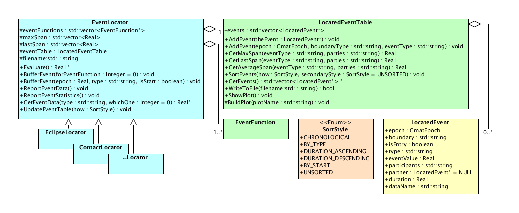
\includegraphics[scale=1.7]{./Images/EventLocator.eps}
\caption{\label{fig:EventLocator}The EventLocator Class and Helpers}
\end{center}
\end{figure} 

Figure~\ref{fig:EventLocator} shows the EventLocator class and the classes that
help it perform its functions.  The EventLocator class acts as the interface
between event function computations, located event data, and the rest of GMAT. 
EventLocator is a base class, providing interfaces to specific event types
through derived classes.  Examples of these derived classes are the
EclipseLocator class and the ContactLocator class, which implement connections
to the event functions needed for eclipses (umbra, penumbra, and antumbra) for
the EclipseLocator, and station rise and set times for the ContactLocator. 
Additional subclasses can be constructed to provide additional event
calculations as needed. 

Each EventLocator contains a LocatedEventTable which stores the data for event
boundaries as they are found.  Located event boundaries are stored in records
in the LocatedEventTable, one per event entry or exit condition.  These records
are stored in the LocatedEvent structure; there is one LocatedEvent for each
entry or exit.  Entry and exit conditions are linked together using the partner
attribute of the LocatedEvent structure.  The LocatedEventTable handles the
presentation of event data to GMAT (and thus to GMAT users).  It provides
methods for sorting and grouping the data, for writing the data to file, and
for accessing event statistics like the maximum, average, and most recent event
durations.  The LocatedEventTable provides several ways to sort event data. 
These sorting options are defined in the SortStyle enumeration.

The EventLocator has the following key attributes and methods\footnote{Note
that while the methods described in this text identify event types and
boundary types as std::string parameters, the implementation may replace the
string representations with Integer identifiers to improve performance.  This
difference in implementation might not be initially available for use, but is
planned for incorporation after the core functionality is in place.}:

\subsubsection{EventLocator Attributes}

\begin{itemize}
\item \textbf{std::vector\textless EventFunction*\textgreater eventFunctions}:
The collection of event functions used by the EventLocator.
\item \textbf{Real *earlyBound}: The early in epoch bound on the event function zero.  This value is used to ensure that the search does not break the bounding points found prior to searching for a function zero.
\item \textbf{Real *lateBound}: The late in epoch bound on the event function zero.  This value is used to ensure that the search does not break the bounding points found prior to searching for a function zero.
\item \textbf{std::vector\textless Real\textgreater  maxSpan}: The longest event
duration encountered by the EventLocator.  There is one entry in this vector per
event function.
\item \textbf{std::vector\textless Real\textgreater  lastSpan}: The most recent
event duration encountered by the EventLocator.  There is one entry in this
vector per event function.
\item \textbf{LocatedEventTable eventTable}: The LocatedEventTable for the
EventLocator.
\item \textbf{std::string filename}: Name of the event data file.
\item \textbf{bool isActive}: Flag used to enable or disable an EventLocator.
\item \textbf{bool showPlot}: Flag used to enable or disable the plot of event data.
\item \textbf{Real eventTolerance}: The tolerance used to determine is an event function zero was located.
\end{itemize}

\subsubsection{EventLocator Operations}

\begin{itemize}
\item \textbf{Real *Evaluate(GmatEpoch atEpoch = -1.0, Real *forState = NULL)}: Evaluates the contained EventFunctions and returns their values and derivatives.  The atEpoch and forState parameters are used during propagation to pass the stage data from the numerical integrator to the EventLocator.  If these parameters are omitted, the locator accesses the data from the target Spacecraft in the event function computations.
\item \textbf{void BufferEvent(Integer forEventFunction)}: Collects data
from an owned event function and adds it to the LocatedEventTable.
\item \textbf{void BufferEvent(Real epoch, std::string type, bool isStart)}:
Adds an event to the LocatedEventTable.
\item \textbf{void ReportEventData()}: Writes the event data to file.
\item \textbf{void ReportEventStatistics()}: Writes the event data statistics
to file.
\item \textbf{Real GetEventData(std::string type, Integer whichOne = 0)}:
Retrieves data for a specified event.  GMAT can access event durations, start
and end times, and other data using this call.
\item \textbf{void UpdateEventTable(SortStyle how)}: Sets or changes the order
of the data in the LocatedEventTable reports.
\end{itemize}

\subsection{EventLocator Helpers}

The EventLocator uses an enumeration and helper class, described here, to track
and sort event data.

\subsubsection{The LocatedEventTable Class}

The core EventLocator helper class is the LocatedEventTable, which acts as a
database of located events for the EventLocator that owns it.  The
LocatedEventTable class has one core attribute: 
\begin{itemize}
 \item \textbf{std::vector\textless LocatedEvent*\textgreater events}: The
event entry and exit data.
\end{itemize}
\noindent It manipulates the vector of events through
the following methods:

\begin{itemize}
\item \textbf{void AddEvent(LocatedEvent *theEvent)}: Adds the passed in event
entry to the table of events.
\item \textbf{void AddEvent(GmatEpoch epoch, std::string boundaryType,
std::string eventType)}: Adds a new event entry to the table of events.
\item \textbf{Real GetMaxSpan(std::string eventType, std::string parties)}:
Returns the longest duration for the detected events of the specified type
involving the specified participants.
\item \textbf{Real GetLastSpan(std::string eventType, std::string parties)}:
Returns the duration of the most recent detected event of the specified type
involving the specified participants.
\item \textbf{Real GetAverageSpan(std::string eventType, std::string parties)}:
Returns the average duration for the detected events of the specified type and
participants.
\item \textbf{void SortEvents(SortStyle how, SortStyle secondaryStyle)}:
Sets flags to sort the event data in the specified primary and secondary order
when generating the event data file.
\item \textbf{std::vector\textless LocatedEvent*\textgreater  *GetEvents()}:
Accessor function that allows for retrieving the event data directly.  This
method provides access to internally managed data, and should be used only when
absolutely necessary.
\item  \textbf{bool WriteToFile(std::string filename)}: Writes the event data
to an event data file with the specified name.
\item \textbf{void ShowPlot()}: Displays a scatter plot of the event data.
\item \textbf{void BuildPlot(std::string plotName)}:  Constructs the scatter
plot of event data and populates the plot data.
\end{itemize}

Each event datum is managed in a LocatedEvent object in the LocatedEventTable. 
The LocatedEvent objects are instances of a structure with the following
attributes:

\begin{itemize}
\item \textbf{GmatEpoch epoch}: The epoch of the data element.
\item \textbf{std::string boundary}: Identifier for the type of datum
represented -- either an entry or exit point.  The boundary string is set by
the event function.  Examples of this string are ``Entry'' or ``Exit'' for
shadow events, and ``Rise'' or ``Set'' for station contact events.
\item \textbf{bool isEntry}: Flag indicating if the event boundary is the start
-- that is, earliest in epoch -- of the span of the event.
\item \textbf{std::string type}: The type of the event, as used in the event
data report and on the scatter plot.
\item \textbf{Real eventValue}: The value of the event function at the reported
event boundary epoch.  This value should have a magnitude less than the
tolerance of the owning EventLocator.
\item \textbf{std::string participants}: The concatenated list of participants
in the event.
\item \textbf{LocatedEvent *partner}: The boundary event on the other side of
the event span.  This pointer is NULL if the span has no matching partner.
\item \textbf{Real duration}: The time, in seconds, of the interval for the
event.
\item \textbf{std::string dataName}: The full name of the event as reported on
the scatter plot and report.  This string is a concatenation of the event type
with the participants string.
\end{itemize}

The event data can be sorted in several different ways\footnote{The sorting functions have not been coded in GMAT R2012a.}.  The sorting options
are controlled using the SortStyle enumeration, which has the following values:

\begin{itemize}
\item \textbf{CHRONOLOGICAL}: Sorts the event data in time order.
\item \textbf{BY\_TYPE}: Groups the data by event type.
\item \textbf{DURATION\_ASCENDING}: Groups the event data by event duration,
from shortest to longest.
\item \textbf{DURATION\_DESCENDING}: Groups the event data by event duration,
from longest to shortest.
\item \textbf{BY\_START}: Arranges data by start epoch, so that the earlier
events occur before later events.
\item \textbf{UNSORTED}: Performs no sorting, so events are reported in the
order they appear in the LocatedEventTable.
\end{itemize}

Subclasses of the EventLocator class differ primarily in the number and type of
EventFunction objects they support.  For example, the first two subclasses of
the EventLocator base are the EclipseLocator and the ContactLocator.  The
EclipseLocator supports three event functions: the Umbra, Penumbra, and
Antumbra Eclipse EventFunction classes.  The ContactLocator supports a single
event function, built in the Contact EventFunction class.  For each supported
EventFunction, the Locator class builds an instance of the class for each set
of participants that can trigger events.  

As an example, an EclipseLocator defined by this scripting:

\begin{quote}
\begin{verbatim}
Create EclipseLocator ecl;
ecl.Spacecraft = {aqua, trmm};
ecl.OccultingBodies = {Earth, Luna};
\end{verbatim}
\end{quote}

\noindent creates twelve EventFunctions; one each for aqua-Earth Umbra,
aqua-Earth Penumbra, aqua-Earth Antumbra, aqua-Luna Umbra, aqua-Luna Penumbra,
aqua-Luna Antumbra, trmm-Earth Umbra, trmm-Earth Penumbra, trmm-Earth Antumbra,
trmm-Luna Umbra, trmm-Luna Penumbra, and trmm-Luna Antumbra.  The EventLocator
base class provides the infrastructure to manage this collection of
EventFunctions; the derived class EclipseLocator provides the details and
instances that provide the functionality.

The EventFunction class defines the computational elements that are necessary
for event location; we examine that class hierarchy next.

\subsection{The EventFunction Classes}

\begin{figure}[ht]
\begin{center}
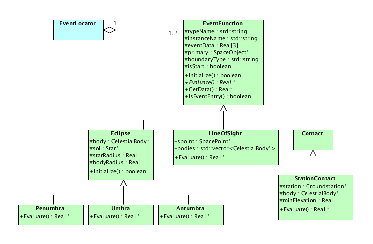
\includegraphics[scale=1.7]{./Images/EventFunction.eps}
\caption{\label{fig:EventFunction}The EventFunction Classes}
\end{center}
\end{figure} 

Event detection is preformed by finding the zeroes of a function defining each
event being analyzed.  The event functions used in GMAT are defined as analytic
functions through at least the first derivative.  These functions are
implemented in classes derived from the EventFunction base class.  The base
class defines the interfaces used by the EventLocator, but leaves the type
specific implementations to the derived classes.  The core interface the
EventLocator needs is the Evaluate() method, which sets the EventFunction value
and first derivative based on the current state of the objects used in the
event function calculations.

The EventFunction base class has the following attributes and methods:

\subsubsection{EventFunction Attributes}

\begin{itemize}
\item \textbf{std::string typeName}: Type of the event.
\item \textbf{std::string instanceName}: Identifier for the specific instance. 
This string is usually set to the concatenated participant list.
\item \textbf{Real *eventData}: The value of the event epoch, event function,
and function derivative with respect to time when last evaluated.  This attribute is allocated dynamically so that composite events -- for example, Contact -- can be coded as a collection of simpler events -- Line of Sight and Elevation for the Contact composite event.
\item \textbf{UnsignedInt datasize}: The size of the eventData vector.
\item \textbf{SpaceObject *primary}: The SpaceObject that plays the role of the
``target'' object in the event function computations.  This role is usually
played by a Spacecraft.
\item \textbf{SpacePoint *origin}: The origin body for the state data.
\item \textbf{boundaryType}: String indicating if the boundary was an entry or
exit.  This string is used in the report and scatter plot, and may vary based on
the type of event being reported.
\item \textbf{bool isStart}: Flag indicating if the event data is at the entry
side of the event function or at the exit side.  This flag is usually set based
in the sign of the most recent function derivative, but can be changed as
needed for specific event functions. 
\end{itemize}

\subsubsection{EventFunction Operations}

\begin{itemize}
\item \textbf{bool Initialize()}: Prepares the event function for use in event
calculations.
\item \textbf{Real* Evaluate()}: Computes the value of the event function and
its derivative.  At the base class level, this method is defined but not
implemented, making it abstract (i.e. ``pure virtual'' in C++).
\item \textbf{Real* GetData()}: Retrieves the most recently computed values of
the event function epoch, value, and derivative.
\item \textbf{bool IsEventEntry()}: Method used to check the event boundary to
see it is is on the entry or exit side of the event function.
\end{itemize}

At this writing, there are three derived EventFunction classes planned for
incorporation into GMAT.  Shadow calculations are performed using the Eclipse
event functions, implemented as 3 subclasses for penumbral, umbral, and
antumbral computations.  Line of sight visibility between a SpacePoint and the
target SpaceObject that takes into account obscuration by intervening bodies is
handled in the LineOfSight subclass. Contact between two SpaceObjects is
performed in the Contact subclasses.  Each of these subclasses contains internal
attributes specific to their computations, as described below.  The leaf level
classes also implement the Evaluate() method to perform the computations
specific to their event computations.  

\subsubsection{Eclipse Event Function Attributes and Operations}

\begin{itemize}
\item \textbf{CelestialBody *body}:  The body casting shadows for these
calculations.
\item \textbf{Star *sol}: The Sun.
\item \textbf{Real starRadius}:  The radius of the Sun.
\item \textbf{Real bodyRadius}:  The shadow body's radius.
\item \textbf{bool Initialize()}: Initialization method for the eclipse data.
\end{itemize}

\noindent The Eclipse EventFunction has three child classes, implementing the
computations for Umbra, Penumbra, and Antumbra shadows.

\subsubsection{LineOfSight Event Function Attributes}

\begin{itemize}
\item \textbf{SpacePoint *spoint}:  The object that is being evaluated along the
line of sight of the target SpaceObject.
\item \textbf{std::vector\textless CelestialBody*\textgreater}:  The celestial
bodies that may lie between the target and the second SpacePoint.
\end{itemize}

\subsubsection{StationContact Event Function Attributes}

The StationContact event function is derived from a Contact intermediate class.
 At this writing, the Contact class is a place holder, and will be filled in
and the StationContact refactored when a second type of contact EventFunction
is defined.

The core attributes of the StationContact class are

\begin{itemize}
\item \textbf{Groundstation *station}:  The station that is being evaluated for
contact with the target.
\item \textbf{CelestialBody *body}:  The body on which the station is located.
\item \textbf{Real minElevation}:  The minimum elevation above the horizon for
a valid contact.  (Note that the elevation can be set negative, resulting in
below-the-horizon contacts.)
\end{itemize}

\section{Root Management Classes}

\begin{figure}[ht]
\begin{center}
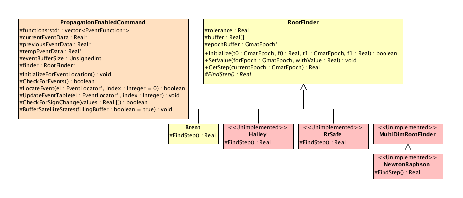
\includegraphics[scale=1.7]{./Images/RootFinders.eps}
\caption{\label{fig:RootFinders}The RootDetector and RootFinder Classes}
\end{center}
\end{figure}

The final classes used in GMAT's event location subsystem are the RootFinder
classes, shown in Figure~\ref{fig:RootFinders}.  These classes are passed to
propagation enabled commands to implement the root monitoring and locating
features of those commands.

\subsection{PropagationEnabledCommand Class Elements}

The PropagationEnabledCommand class monitors the active EventFunctions, watching
for sign changes in the function values and the derivative values during
propagation.  It maintains a set of two element ring buffers of data for each
event function that it is monitoring.  The attributes of the command are
validated and reset as needed at the start of each propagation in the 
command's PrepareToPropagate() and Initialize() methods. 

PropagationEnabledCommands have the following attributes and operations
specific to event detection:

\subsubsection{Root Detection Attributes}

\begin{itemize}
\item \textbf{std::vector\textless{EventFunction*}\textgreater functions}: Table
of active EventFunction objects.  
\item \textbf{Real *currentEventData}: The epochs, function values, and
derivative values of the data most recently evaluated.
\item \textbf{Real *previousEventData}: The epochs, function values, and
derivative values of the data evaluated immediately prior to the most recent
evaluation.
\item \textbf{Real *tempEventData}: A temporary buffer of event data used when
performming event location tasks.
\item \textbf{UnsignedInt eventBufferSize}: The number of elements in the event
data buffers.
\item \textbf{RootFinder *finder}:  The event finder used to compute steps for
the root finding iterations.
\end{itemize}


\subsubsection{Root Detection Operations}

\begin{itemize}
\item \textbf{void InitializeForEventLocation()}: Initializes the event
location elements of the command.
\item \textbf{bool CheckForEvents()}: Method called to see if an event candidate
exists.
\item \textbf{bool LocateEvent(EventLocator *el, Integer index = 0)}: Search
driver used to find event boundaries.
\item \textbf{void UpdateEventTable(EventLocator *el, Integer index)}: Method
that triggers storage or removal of event boundary data in the located event
table of an event locator.
\item \textbf{bool CheckForSignChange(Real[] values)}:  Tester to see if a
potential event candidate exists for a set of values.
\item \textbf{void BufferSatelliteStates(bool fillingBuffer = true)}: Buffers
and restores SpaceObject data so that the propagators can perform searches
without disturbing the main propagation data.
\end{itemize}

\subsection{The RootFinder Class}

The RootFinder class is a base class that defines the root solving interfaces
used by the propagation enabled commands.  It works with teh propagation
enabled command's LocateEvents() method to step the propagation state vector to
specific epochs and then evaluate candidate EventFunctions.  The resulting
function values are then compared to a specified tolerance value, and if within
that tolerance of zero, declared as a located root of the EventFunction. 

Derived classes implement the FindStep method, which implements algorithm
specific ways of finding the epochs for the propagation.

\subsubsection{RootFinder Attributes}

\begin{itemize}
\item \textbf{Real tolerance}: The tolerance for the event location test.
\item \textbf{Real *buffer}: Buffer of event function or function derivative
values used by the root finding algorithm.
\item \textbf{GmatEpoch *epochBuffer}: Buffer of corresponding epoch values.
\end{itemize}

\subsubsection{RootFinder Operations}

\begin{itemize}
\item \textbf{bool Initialize(GmatEpoch t0, Real f0, GmatEpoch t1, Real f1)}:
Prepares the root finder to search for a root by passing in the bracketing
function epochs and values.
\item  \textbf{void SetValue(GmatEpoch forEpoch, Real withValue)}: Passes in a
new epoch and related value during the root search.
\item \textbf{Real GetStep(GmatEpoch currentEpoch)}: Access routine to retrieve
the step to the next epoch.  This method calls FindStep(), which implements teh
algorithm specific step size computations.
\item \textbf{Real FindStep()}:  Implements the time step calculation
algorithm.  This method is defined but not implemented in the RootFinder base
class, making it abstract (``pure virtual'' in C++),
\end{itemize}

\subsubsection{The Brent Class}

The Brent class implements Brent's method\cite{numrec} to determine the time
step to a candidate root location.  It implements a single core method:

\begin{itemize}
\item \textbf{Real FindStep()}:  Implements Brent's method to determine
candidate time steps for root location.
\end{itemize}

\section{Known Issues}

The current implementation of the event location subsystem, delivered with R2012a, is provided as a GMAT plug-in.  The plug-in code is considered an alpha release because of the following issues uncovered during test, but not yet corrected.

\begin{itemize}
\item \textbf{Backwards Propagation} Event location during backwards propagation does not collect the event data correctly.  This issue has been reported as issue GMT-421.
\item \textbf{Solver Reporting} Events located in a solver control sequence are reported multiple times as they are found during the solver iterations.  The desired behaviour -- reporting only for the final nominal run -- is not yet implemented. This issue has been reported as issue GMT-4.
\item \textbf{Formation Propagation}  Event location integration causes a crash when spacecraft are propagated in a formation.  This issue has been reported as issue GMT-335.
\item \textbf{SPK Propagation Errors}  If the SPICE propagator encounters an error during propagation when event location is also being performed, GMAT will crash.  This issue has been reported as issue GMT-391.
\item \textbf{Bad Propagation Steps}  This issue has been reported as issue GMT-376 and GMT-378.
\item\textbf{Incorrect Origin}  In cases where the propagation origin changes during event location, the radius of the original origin body is being used in checks to see if the current location is inside of the obscuring body.  This results in a report that the state is bad, even in cases where it is actually good.  This issue has been reported as issue GMT-377.
\item \textbf{Eclipses and Ephemerides}  During event location, the ephemeris file interpolator is being passed non-monotonic data if we event location is active.  This issue has been reported as issue GMT-173.
\item \textbf{Eclipses and Finite Burns}  Event location cannot be performed during finite burns because of an initialization issue in the propagation subsystem.  This issue has been reported as issue GMT-334.
\item \textbf{Performance Issues}  Event location should be tuned to perform better during a run.  This issue has been reported as issue GMT-255.
\item \textbf{Location Tolerances}  The accuracy of the event location algorithm is based on the value of the event function, which is not an easily interpreted value for the users.  It should be specified in units of time instead.  This issue has been reported as issue GMT-422.
\item \textbf{Derivative Zero Checks}  The derivative zero location code is in place, but not activated for R2012a.  The function zero location code for derivatives is not yet coded.  These pieces need to be completed.  This issue has been reported as issue GMT-457. 
\item \textbf{Sorting is not implemented}  The sorting described in the enumeration of sort styles is not yet implemented.  This issue has been reported as GMT-496.
\end{itemize}

\begin{thebibliography}{10}

\bibitem{pip}Joel J. K. Parker, \emph{A General Event Location Algorithm with
Applications to Eclipse and Station Line-of-Sight}, NASA Goddard Space Flight
Center, 2011, PIP Final Report.

\bibitem{aasastro}Joel J. K. Parker and Stephen P. Hughes, \emph{A General
Event Location Algorithm with Applications to Eclipse and Station
Line-of-Sight}, Proceeding of the AAS/AIAA Astrodynamics Specialist Conference,
AAS 11-527, 2011.

\bibitem{archspec}GMAT Development Team, \emph{General Mission Analysis Tool
(GMAT) Architectural Specification}, R2011a Draft, April, 2011.

\bibitem{numrec}William H. Press, Saul A. Teukolsky, William T. Vetterling, and
Brian P. Flannery, \emph{Numerical Recipes}, Cambridge University Press, Third
Edition, 2007.

\end{thebibliography}

\end{document}
